\documentclass[a4paper,11pt,uplatex]{jsarticle}
\usepackage{amsmath,amssymb}
\usepackage{bm}
\usepackage[dvipdfmx]{graphicx}
\usepackage{here}
\usepackage{multirow}

%テキストの表示領域の調節
\setlength{\textwidth}{\paperwidth}
\addtolength{\textwidth}{-40truemm}
\setlength{\textheight}{\paperheight}
\addtolength{\textheight}{-45truemm}

%余白の調節
\setlength{\topmargin}{-10.4truemm}
\setlength{\evensidemargin}{-5.4truemm}
\setlength{\oddsidemargin}{-5.4truemm}
\setlength{\headheight}{17pt}
\setlength{\headsep}{10mm}
\addtolength{\headsep}{-17pt}
\setlength{\footskip}{5mm}


% \nofiles
\begin{document}
\section{目的}
機械構造用材料として使用される金属材料の代表例として,鋼とアルミニウム合金を用いて金属組織と機械的特性について理解することを目的とする.
金属組織観察では,熱処理として,焼きなまし,焼入れ,焼入れ焼きもどしを施した各種炭素鋼の組織を光学顕微鏡で観察し,
熱処理によって組織がどのように変化するかを学ぶ.また,低炭素鋼とアルミニウム合金の引張試験を行い,引張試験から得られる機械的特性について学ぶ.

\section{金属材料の組織観察}
\subsection{目的}
金属材料の性質の分類として,金属組織に対して鈍感な性質(組織鈍感性)と敏感な性質(組織敏感性)の2つに大別することがある.
前者の代表例は比重,比熱,縦弾性係数,横弾性係数などが挙げられ,これらは金属組織あるいはその微細構造に比較的鈍感であるという性質を持つ.
後者の代表例は,降伏応力,引張強度,破断伸びなどの機械的特性などが挙げられ,これらは金属組織あるいはその微細組織に最も敏感である.
そのため,機械材料の性質判定の重要な手段として,古くから光学顕微鏡による組織観察が用いられてきた.
最近では,走査型電子顕微鏡,透過型電子顕微鏡による組織観察を行い,組織と金属材料の特性との関係が研究されている. 
熱処理は,金属材料の性質を改善するために行う加熱,冷却の操作であるが,特に鋼では変態現象を利用した加熱,冷却の熱処理によってその性質は大きく変化し,
この熱処理の効果は合金化によって極めて大きな変化を示すことがある.従って熱処理は鋼を取り扱う上で極めて重要である. 
また,鋼は他の金属材料と比較して大量生産が容易,価格が安いことから非常に重要な金属材料で,用途が広く使用量も極めて多い.
そこで,金属組織の観察では,炭素鋼を試料として用い,焼きなまし,焼入れ,焼入れ焼もどしの熱処理を施した試料表面の組織を観察し,
組織の種類,配置分布,形状,大きさとこれらの相互関係を調べると共に,熱処理による組織の変化について学ぶ.これが本実験の目的である.

\subsection{Fe-Cの平衡状態図と熱処理}
\begin{figure}[H]
  \begin{tabular}{cc}
    \begin{minipage}{0.5\hsize}
      \begin{center}
        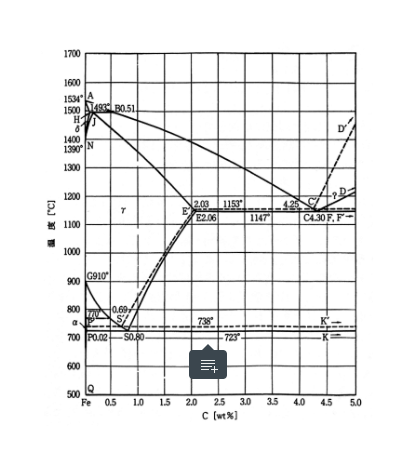
\includegraphics[width = 5cm]{画像/FeC平衡図.png}
        \caption{Fe-Cの平衡状態図}
        \label{FeC平衡図}
      \end{center}
    \end{minipage}

    \begin{minipage}{0.5\hsize}
      \begin{center}
        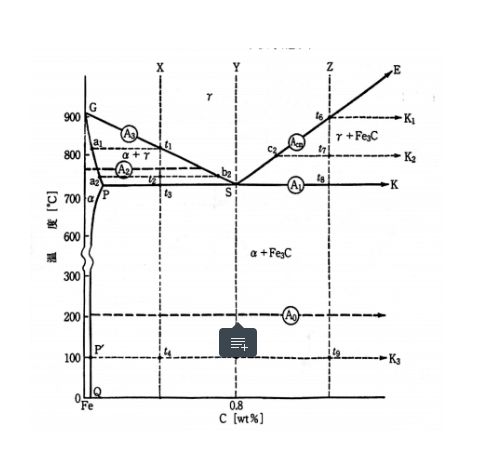
\includegraphics[width = 5cm]{画像/FeC平衡図拡大.png}
        \caption{Fe-Cの平衡状態図(拡大)}
        \label{FeC平衡図拡大}
      \end{center}
    \end{minipage}
  \end{tabular}
\end{figure}

図\ref{FeC平衡図}は,Fe-C系平衡状態図,図\ref{FeC平衡図拡大}はFe-C系平衡状態図の一部を拡大したものである.
平衡状態図は,ある炭素濃度の鋼をある温度で保持したときの組織を示すものである. 
鋼を均一オーステナイト状態まで加熱・保持した後,炉内でゆっくり冷却する処理を焼きなましと呼び,この時得られる組織を標準組織という.
標準組織の鉄鋼は次式で与えられる引っ張り強さ$\sigma B$を示すことが知られている.
\begin{align}
  \sigma B=  281\times(1−\frac{C\%}{0.8})+  830\times(\frac{C\%}{0.8}) [\mathrm{MPa}]
\end{align}
ここで,281Mpaはフェライト自体の引っ張り強さ,830Mpaはパーライト自体の引張強さである. 
焼ならしは,焼きなまし処理と同様に鉄鋼を均一オーステナイト状態まで加熱・保持した後,空気中で自然冷却する熱処理で,その結果得られる組織をソルバイトと呼び.
強さと靭性の優れた鉄鋼材が得られる.図\ref{機械的特性}は焼きなましと焼ならしを施した鉄鋼の機械的特性と炭素量の関係を示す.
一方,機械構造用部品等に要求される強さと靭性は焼ならしでは十分に得られない場合があり,この場合は焼入れ焼きもどしによって組織を改善する必要がある.
焼入れは,鉄鋼を均一オーステナイト状態まで加熱・保持した後,水中に炭素鋼を入れて急冷する熱処理である.
焼入れしたままの鉄鋼は非常に硬いが反面非常にもろく,そのままでは実際の仕様に耐えない場合が多い.
そこで焼入れ後100°CからA1点直下(オーステナイトを生じない温度)まで再加熱し冷却する熱処理を焼きもどしと呼ぶ.
焼戻しによって,鉄鋼はソルバイトあるいはトルータイトの組織になる.


\begin{figure}[H]
  \begin{tabular}{cc}
    \begin{minipage}{0.5\hsize}
      \begin{center}
        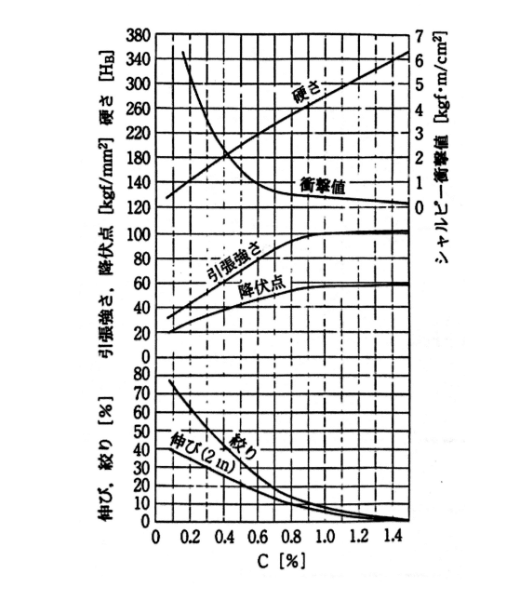
\includegraphics[width = 5cm]{画像/機械的特性.png}
        \caption{機械的特性と炭素量の関係}
        \label{機械的特性}
      \end{center}
    \end{minipage}

    \begin{minipage}{0.5\hsize}
      \begin{center}
        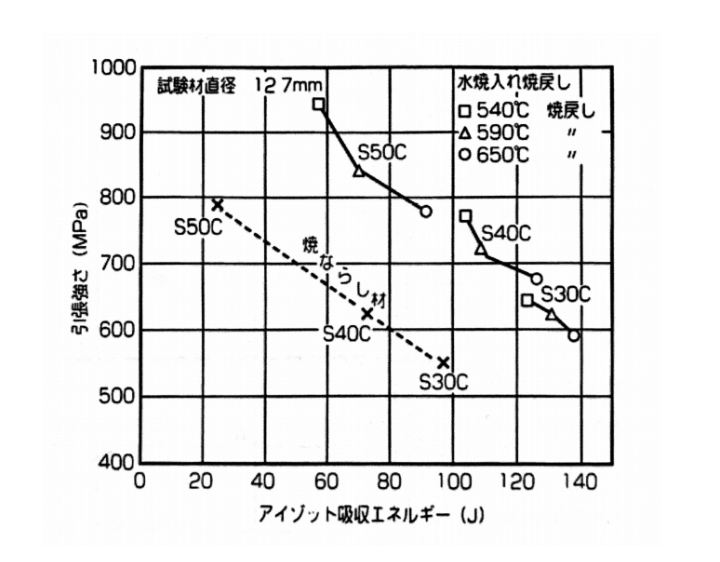
\includegraphics[width = 5cm]{画像/引張強度の比較.png}
        \caption{焼ならし材と焼入れ焼もどし材の引張強度の比較}
        \label{引張強度の比較}
      \end{center}
    \end{minipage}
  \end{tabular}
\end{figure}
図\ref{引張強度の比較}は機械構造用炭素鋼S30C,S40C,S50Cの焼ならし材と焼入れ焼きもどし材の引張強度をアイゾット吸収エネルギー(靭性値)の関係で整理したものである.
焼入れ焼きもどし材は焼ならし材に比べて,引張強度と靭性の点ではるかに優れていることがわかる.
以上より,鉄鋼の組織と機械的特性とは密接に関係しており,目的に応じた性質の鉄鋼を得るために各種の熱処理が行われている.

\subsection{純鉄の変態と組織}
図\ref{FeC平衡図},\ref{FeC平衡図拡大}の平衡状態図上で,純鉄は炭素量がほぼ0\%の箇所となる.図\ref{純鉄の同素変態}より純鉄は912°C以下では体心立格子の結晶構造のフェライト(α鉄)と呼ぶ.
912°C以上では面心立方格子の結晶構造のオーステサイト(γ鉄),1394°C以上では再び体心立方格子にかわり,
δ鉄と呼ぶ.912°Cと1394°Cは同素変態点であり,$A_3$点,$A_4$点という.

\begin{figure}[H]
  \begin{center}
    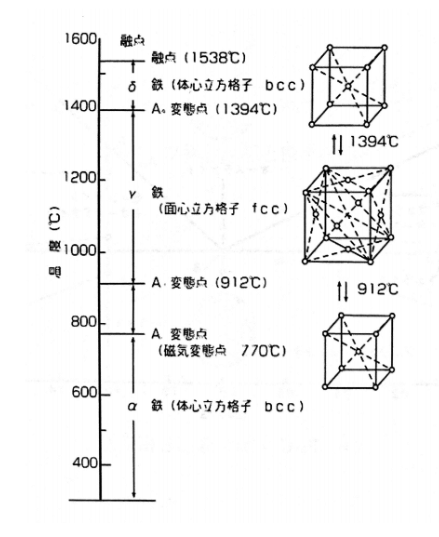
\includegraphics[width = 6cm]{画像/純鉄の同素変態.png}
    \caption{純鉄の同素変態と結晶格子}
    \label{純鉄の同素変態}
  \end{center}
\end{figure}

\subsection{平衡状態図と相変態}
純鉄と異なり炭素を含有する炭素鋼の相変態について説明する.オーステナイト状態から焼きなましを行い,
平衡状態図にほぼ従って形成した組織を2.2節で説明したように標準組織という.図\ref{相変態}に標準組織の生成過程と起こる組織変化を平衡状態図で示す.
\begin{enumerate}
  \item 炭素量が0.4\%の炭素鋼をXの温度から焼きなましした場合,$A_3$線上の高温ではオーステナイトであるが,$T_1$の温度($A_3$線上)で,
  炭素濃度$\alpha_1$のフェライトの析出が始まる.$A_3$から$A_!$で析出したフェライトを初析フェライトという. さらに温度が低下するとフェライト量が次第に増加し,
  オーステナイト量は減少する. フェライトは0.02\%しか炭素を固溶できないため, 未変態のオーステナイトの炭素量はGS線に沿って次第に増加し, 723℃($A_1$線上)で
  炭素濃度は0.8\%となる.$A_1$点で未変態のオーステナイトが共析変態を起こしてパーライトとなる. パーライトはフェライトとセメンタイトが交互に並んだ層状組織である.
  この時,既に析出していたフェライトは変化せずにそのままであるため, 初析フェライトとパーライトの混合組織になる.

  \item 炭素量が0.8\%の炭素鋼をYの温度から焼きなましした場合,S点に到達するまではオーステナイト単相であるが,
  S点に達すると,オーステナイトはP点で示される炭素濃度のフェライトとセメンタイト($Fe_3C$)に分解する共析変態が起こり, 全てパーライトとなる.

  \item 炭素量が1.2\%の炭素鋼をZの温度から焼きなましした場合,$A_{cm}$線以上の高温ではオーステナイトであるが, $T_6$の温度で($A_{cm}$線上で),
  セメンタイトがオーステナイトの粒界に析出を始める.このセメンタイトは網目状に析出し, これを初析セメンタイトという.
  更に温度が低下すると初析セメンタイト量は増加し,未変態のオーステナイトの炭素量はES線に沿って低下し,723°C($A_1$線上)で炭素濃度は0.8\%となる.
  $A_1$点で未変態のオーステナイトが共析変態を起こしてパーライトとなる.$A_1$点以下の温度では, 網目状のセメンタイトとパーライトの組織となる.

\end{enumerate}

\begin{figure}
  \begin{center}
    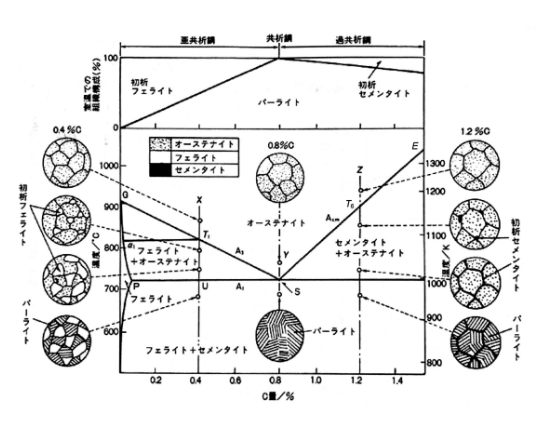
\includegraphics[width = 8cm]{画像/相変態.png}
    \caption{Fe-C平衡状態図と相変態}
    \label{相変態}
  \end{center}
\end{figure}

\subsection{平行状態図と標準組織}
図\ref{標準組織}は純鉄と炭素量が1.4\%までの各種炭素鋼の標準組織を示したものである.
2.4節で説明したように, 炭素量が0.4\%の炭素鋼の標準組織は,白色部のフェライトと黒色部のパーライトからなり,
黒色部のパーライトを拡大すると層状組織となっている.さらに炭素量が増えると黒色部のパーライトが増え,0.8\%の炭素鋼は全てパーライトとなる.
さらに炭素量が増えて1.4\%の炭素鋼では,白色網状のセメンタイト($Fe_3C$)と黒色部のパーライト組織が得られる.

\begin{figure}
  \begin{center}
    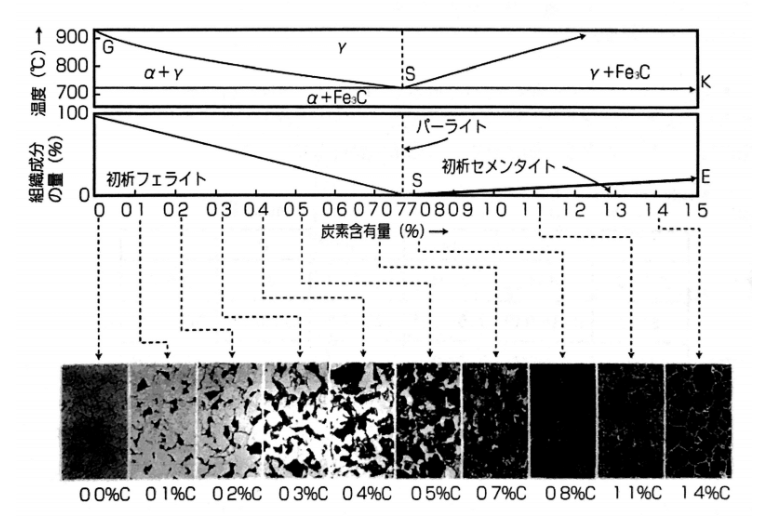
\includegraphics[width = 10cm]{画像/標準組織.png}
    \caption{平衡状態図と標準組織}
    \label{標準組織}
  \end{center}
\end{figure}

\subsection{試料}
炭素鋼の組織観察で使用する5種類の炭素鋼の化学成分と焼きなまし,焼入れ,焼もどしを行った試料の番号との対応を表\ref{化学成分表},\ref{試料の種類}に示す.

\begin{table}[H]
  \begin{center}
    \caption{各種炭素鋼の化学成分表(mass\%)}
    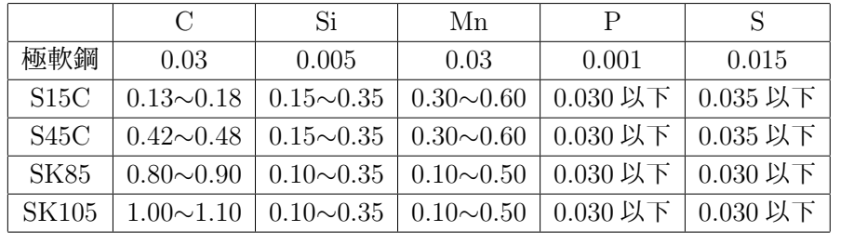
\includegraphics[width = 8cm]{画像/化学成分表.png}
    \label{化学成分表}
  \end{center}
\end{table}

\begin{table}[H]
  \begin{center}
  \caption{組織観察用の試料の種類}
  \label{試料の種類}

  \begin{tabular}{|l|l|l|lll|}
  \hline
                         & No. & 熱処理     &      &                       &                      \\ \hline
  極軟鋼                  & 22  & 焼なまし    & 焼なまし & $\cdots$ & 極軟鋼: 950℃ 30分加熱→炉冷   \\ \cline{1-3}
  S15C                   & 23  & 焼なまし    &      &                       & S15C: 900℃ 30分加熱→炉冷  \\ \cline{1-3}
  \multirow{3}{*}{S45C}  & 24  & 焼なまし    &      &                       & S45C: 850℃ 1時間加熱→炉冷  \\ \cline{2-3}
                         & 25  & 焼入れ     &      &                       & SK105: 950℃ 1時間加熱→炉冷 \\ \cline{2-3}
                         & 26  & 焼入れ焼もどし &      &                       &                      \\ \cline{1-3}
  \multirow{3}{*}{SK85}  & 27  & 焼なまし    & 焼入れ  & $\cdots$ & 850℃ 30分加熱→水焼入れ      \\ \cline{2-3}
                         & 28  & 焼入れ     &      &                       &                      \\ \cline{2-3}
                         & 29  & 焼入れ焼もどし &      &                       &                      \\ \cline{1-3}
  \multirow{3}{*}{SK105} & 30  & 焼なまし    & 焼もどし & $\cdots$ & 焼入れ後, 600℃ 30分加熱→空冷  \\ \cline{2-3}
                         & 31  & 焼入れ     &      &                       &                      \\ \cline{2-3}
                         & 32  & 焼入れ焼もどし &      &                       &                      \\ \hline
  \end{tabular}
\end{center}
\end{table}

\subsection{試料作製と検鏡法}
\subsubsection{研磨}
顕微鏡試料の作成は次の手順で行った.
\\ \\
試料の採取→グラインダー(ヤスリ)研磨→エメリー紙研磨(\#1000→\#1500)→仕上げ研磨(バフ研磨)
\\ \\
本実験では, エメリー紙研磨から始めた. 研磨は1方向に行い, 研磨面に以前の大きな傷が消えたら,
次の細かいエメリー紙による研磨に移行し, 1つ前と直角方向に同様に行う. 以上のように順次細かい研磨紙に移行した.
次に,仕上げ研磨はラシャ布を貼った回転円盤上に,$\mathrm{Cr_2O_3,Al_2O_3,MgO}$などの極めて微細な粉末の混濁液を滴下しながら
試料面が鏡面光沢になるまで研磨を行った.これをバフ研磨という. 本実験では酸化クロム(Ⅲ)($\mathrm{Cr_2O_3}$)を用いてバフ研磨を行った.

\subsubsection{エッチング}
光学顕微鏡では,主に試料面の凹凸の差により起こる反射光の明暗の差によって組織を調べるため,適当な腐食液で腐食する必要がある.
本実験で使用する炭素鋼は,表\ref{エッチング}の腐食液を使用した.試料表面を腐食液に浸し,適切な腐食時間経過後,直ちに試料表面を流水中で水洗した.
この時腐食した表面には絶対触らないこと,水洗いが済んだら直ちに試料表面を乾燥させることを注意した.

\begin{table}[H]
  \begin{center}
  \caption{エッチング}
  \label{エッチング}

  \begin{tabular}{|l|l|l|l|l|l|}
\hline
金属名                 & No.                    & エッチング液(腐食液)                 & 化学成分          & 時間                     & 適用                                                    \\ \hline
\multirow{8}{*}{鉄鋼} & \multirow{5}{*}{22〜30} & \multirow{5}{*}{硝酸アルコール}    & 硝酸1〜5cc       & \multirow{5}{*}{数秒〜1分} & \multirow{5}{*}{炭素鋼の全ての組織, パーライトは黒く着色, フェライト粒界が現出する.} \\
                    &                        &                             & エチルアルコール100cc &                        &                                                       \\
                    &                        &                             & または,          &                        &                                                       \\
                    &                        &                             & 硝酸4〜5cc       &                        &                                                       \\
                    &                        &                             & メチルアルコール100cc &                        &                                                       \\ \cline{2-6}
                    & \multirow{3}{*}{31,32} & \multirow{3}{*}{ピクリン酸アルコール} & ピクリン酸4cc      & \multirow{3}{*}{数秒〜1分} & \multirow{3}{*}{炭素鋼の全ての組織.}                           \\
                    &                        &                             & エチルアルコール または, &                        &                                                       \\
                    &                        &                             & メチルアルコール100cc &                        &                                                       \\ \hline
\end{tabular}
\end{center}
\end{table}

\subsubsection{検鏡}
金属顕微鏡は, 試料面に対して垂直に光を当てて反射光によって観察を行うので, 光軸に対して試料面を垂直におく必要がある.
このために, 試料をスライドガラス上に付着させた油粘土の上に乗せて, 試料平圧器を用いて上から静かに押して試料面がスライドガラス面と平行になるようにした.
このスライドガラスに固定された試料を顕微鏡のステージに乗せて検鏡した.
\par
焦点の合わせ方は対物レンズと試料面が当たることがないように, 10倍程度の低倍率対物レンズを用いて, ピントを合わせ,
次に高倍率の対物レンズに変えて微動ハンドルによりピントを合わせた.
\par
各試料で最適な倍率に設定した後, 顕微鏡にセットしたカメラで撮影した.

\subsection{組織写真}


\section{金属材料の引張試験}
\subsection{目的}
機械,構造物の設計に必要な金属材料の静的な機械的特性を取得するためには,金属材料の引張試験を行う必要がある.
引張試験によって金属材料の弾性と塑性の特性,引張強さ,破断伸び,破断絞りなどの基本的な機械的特性を測定することができる.
そこで,炭素鋼とアルミニウム合金を供試材として引張試験を行い,機械的特性を測定し引張試験方法を修得するとともに,
炭素鋼とアルミニウム合金の機械的特性の違いについて学ぶことを目的とする.
\subsection{引張試験}
引張試験は,金属材料の縦弾性係数, 降伏点,0.2\%耐力,引張強さ,破断伸び,破断絞りなどの機械的特性を測定するために,試験片に引張荷重を加え,
破断に至るまでひずみを与える試験で,この金属材料の引張試験方法はJIS Z 2241「金属材料引張試験方法」で規定されている. 
\par
図\ref{鋼のひずみ}は低炭素鋼の応力-ひずみ線図であり, 引張試験の全行程における試験片平行部の公称応力とひずみの関係を表す曲線である.
図のA点より手前では応力とひずみの間に比例関係があり,その傾きを縦弾性係数(ヤング率),この範囲を弾性域と呼び,応力を0に戻せばひずみも0に戻る.
A点に応力が達すると材料が降伏を開始する.A点を上降伏点と呼ぶ.A点より後は塑性域と呼ぶ.降伏領域を過ぎると加工硬化によって材料の変形抵抗が増加し,
最大応力点(引張強さ)に達する.その後,試験片平行部のある部分でくびれが生じ始めるために,応力が減少し最後に試験片が破断する. 
\par
図\ref{非鉄のひずみ}は非鉄金属や軟鋼以外の鉄鋼(ステンレスなど)の応力-ひずみ線図である.この場合は明瞭な降伏点が現れない.そこで0.2\%の塑性ひずみ
が生じる応力を0.2\%耐力と呼び,降伏点の代わりに用いる

\begin{figure}[H]
  \begin{tabular}{cc}
    \begin{minipage}{0.5\hsize}
      \begin{center}
        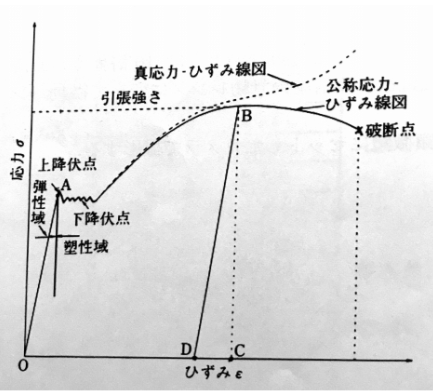
\includegraphics[width = 5cm]{画像/鋼の歪み.png}
        \caption{鋼の応力-ひずみ線図}
        \label{鋼のひずみ}
      \end{center}
    \end{minipage}

    \begin{minipage}{0.5\hsize}
      \begin{center}
        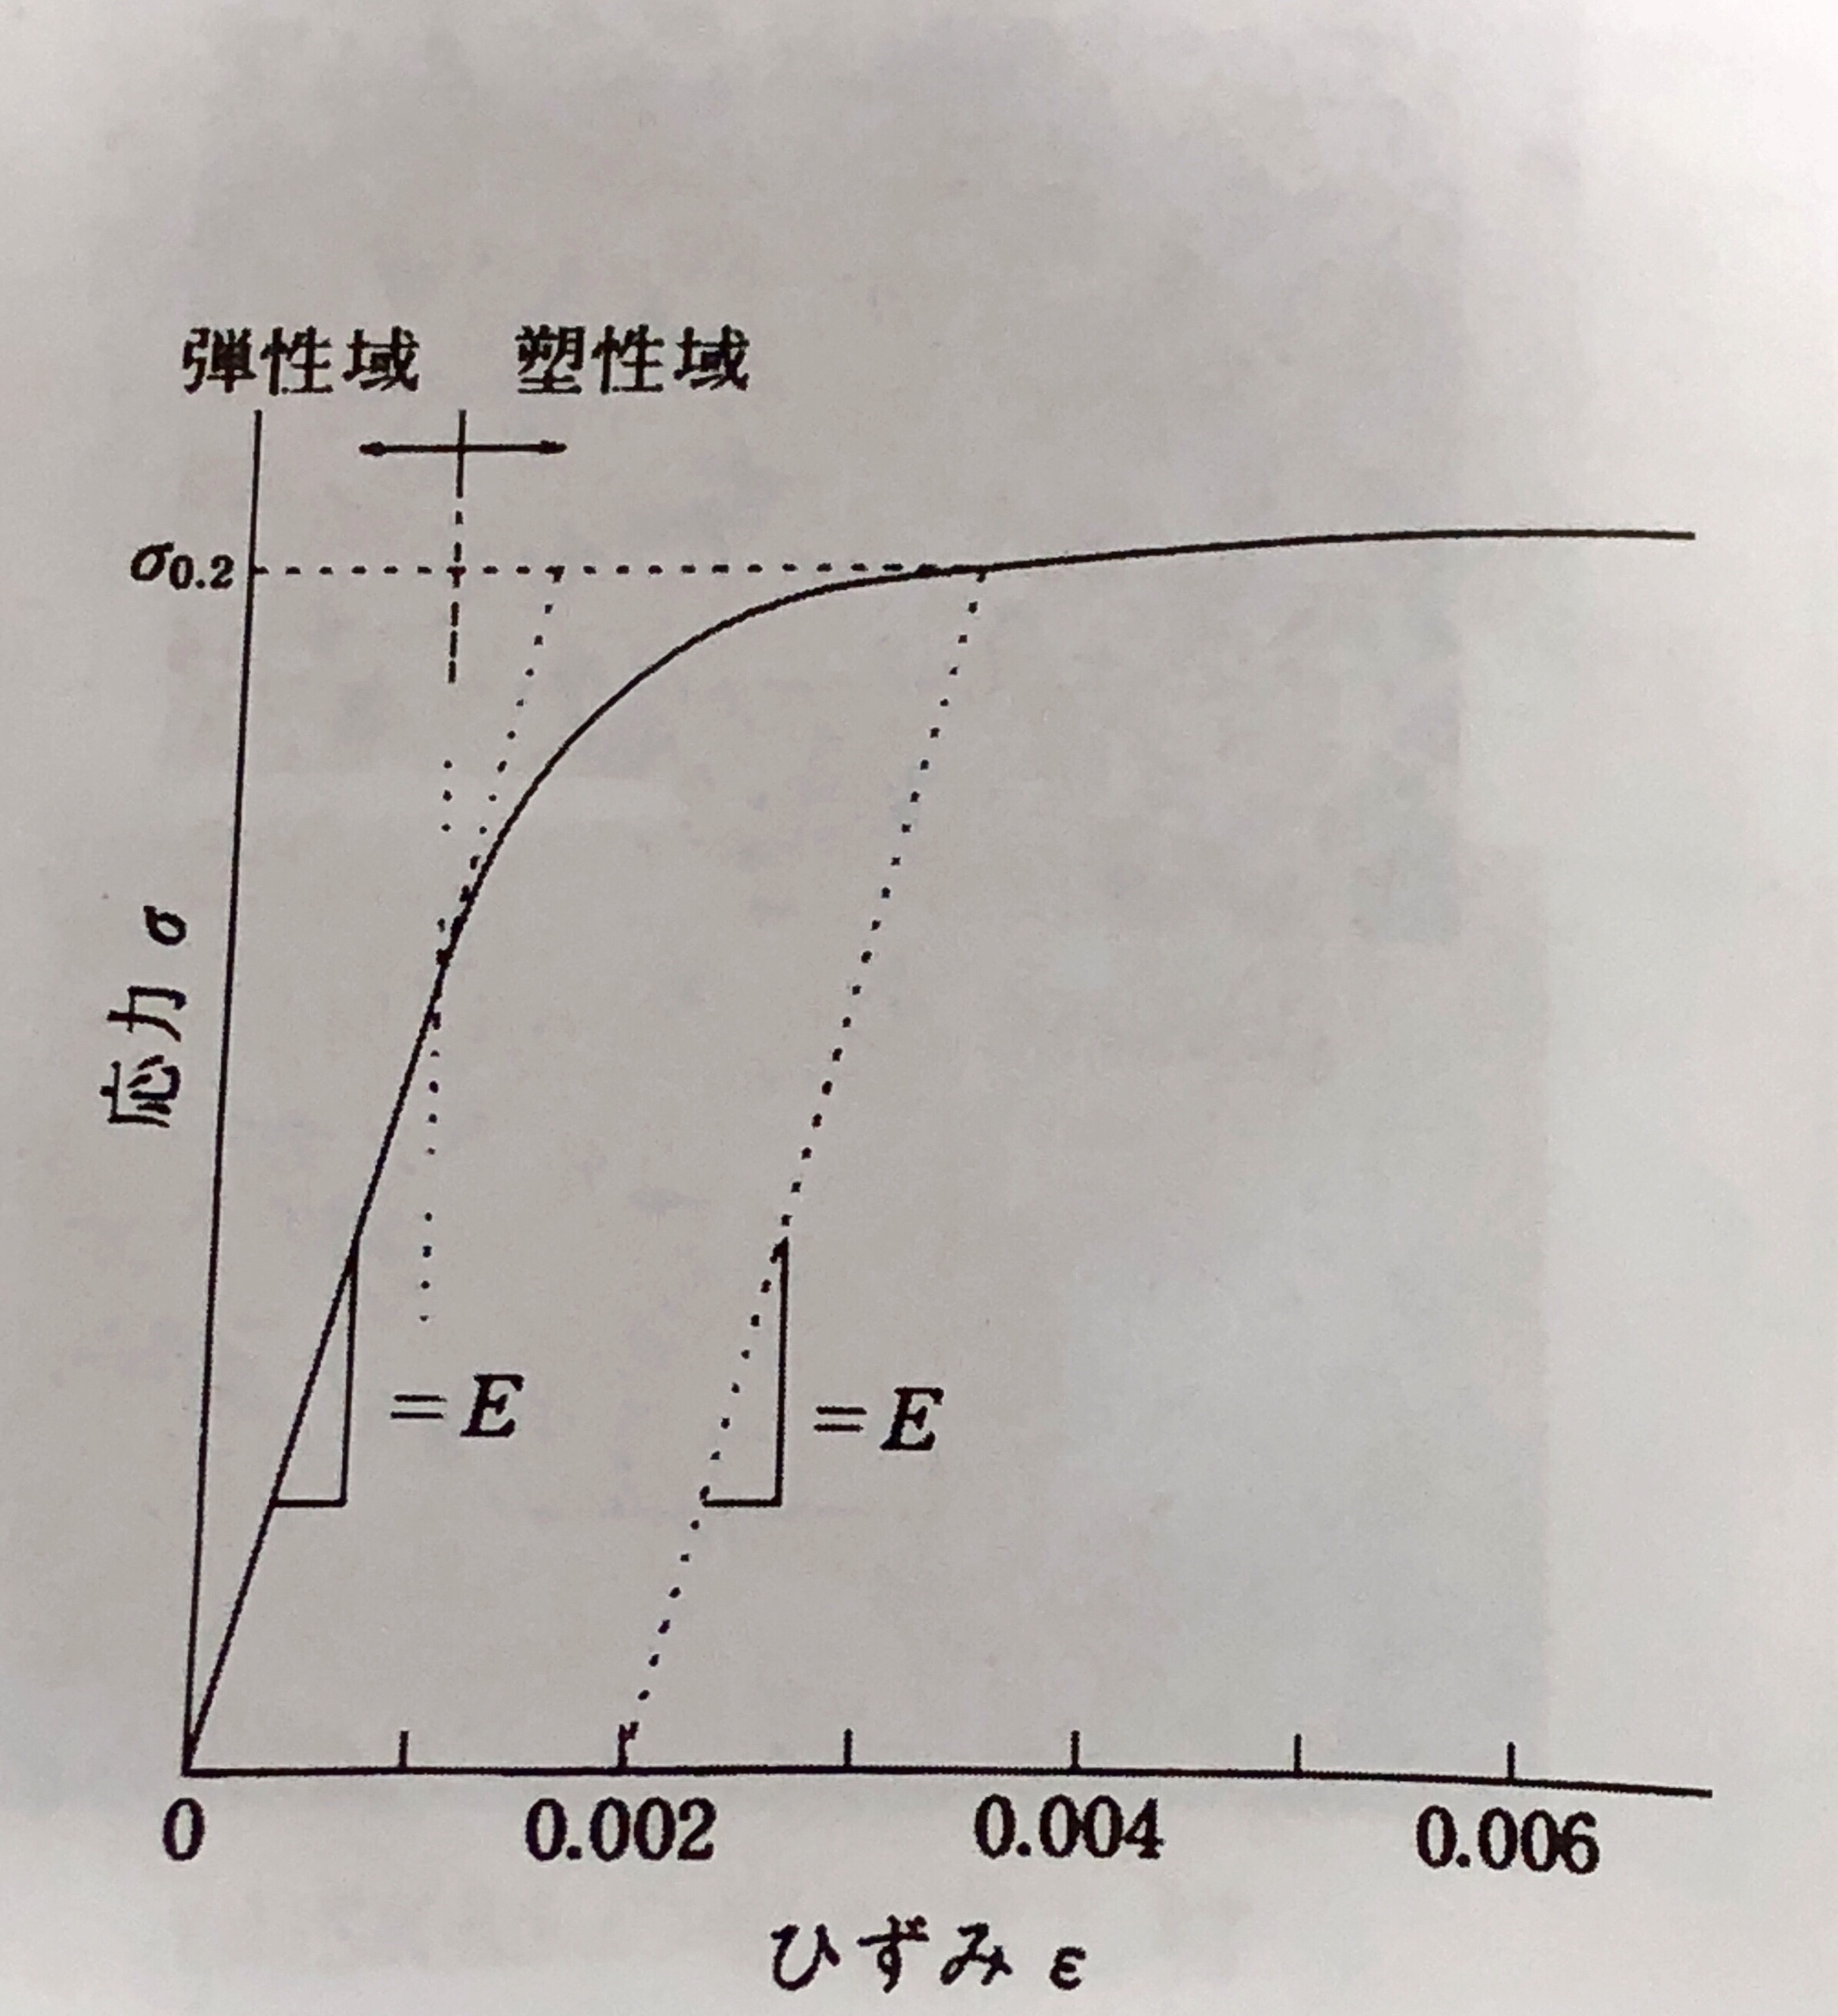
\includegraphics[width = 5cm]{画像/非鉄の歪み.jpg}
        \caption{非鉄金属の応力-ひずみ線図}
        \label{非鉄のひずみ}
      \end{center}
    \end{minipage}
  \end{tabular}
\end{figure}

\subsection{試験装置}
本実験に使用する試験装置は,コンピュータ制御型万能試験機(Istron社製4505またはIstron社製5882)である.
本装置は,実験装置本体,制御装置,PCから構成される.図\ref{試験機}に試験機の構成図を示す.

\begin{figure}[H]
  \begin{center}
    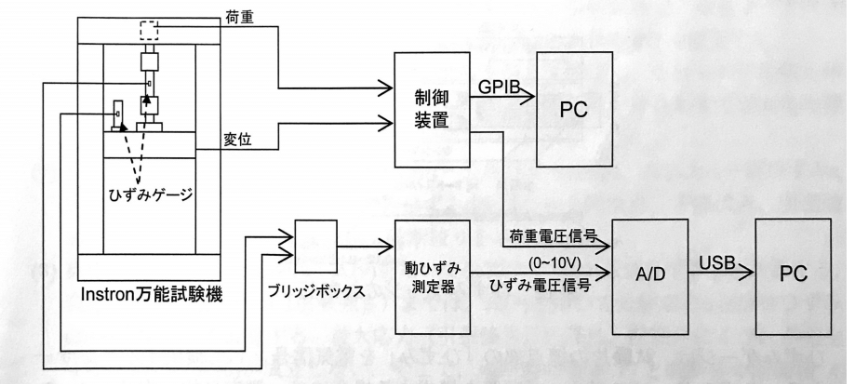
\includegraphics[width = 10cm]{画像/試験機.png}
    \caption{試験機構成図}
    \label{試験機}
  \end{center}
\end{figure}

\subsection{供試材}
引張試験の供試材はA1100(アルミニウム合金)と900°C,1hourで焼きなまししたSPCC(冷間圧延鋼板)である.
供試材の化学成分を表\ref{化学成分表2}に示す.試験片の形状はJIZ2241(金属材料引張試験方法)で規定されている13B号試験片を用いる.
図\ref{試験片}に試験片の形状寸法を示す.

\begin{table}[H]
  \begin{center}
    \caption{化学成分表(mass\%)}
    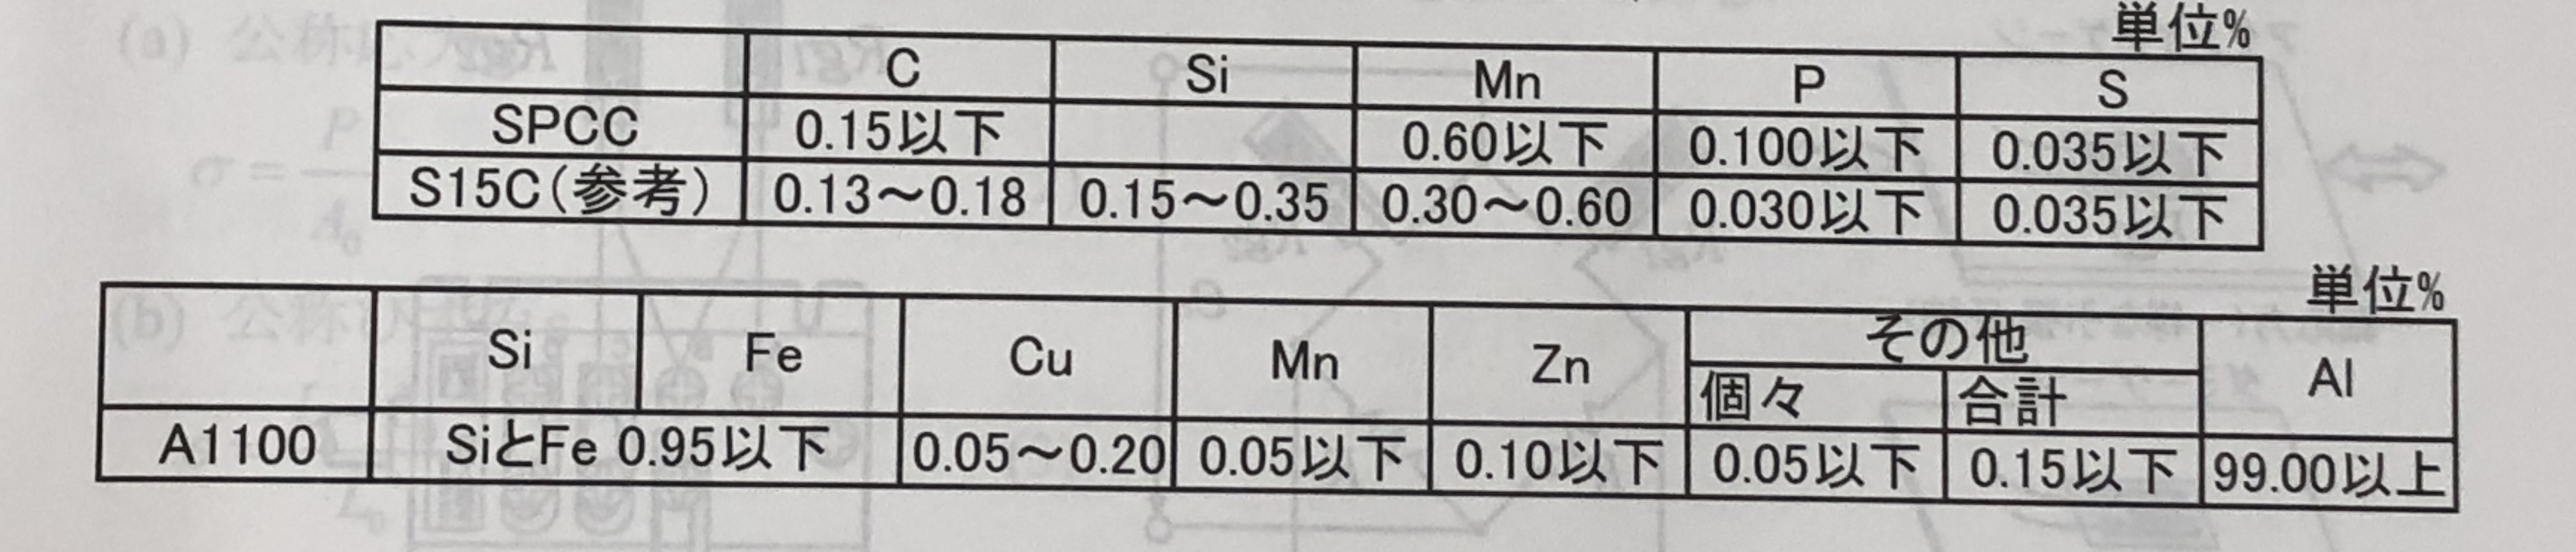
\includegraphics[width = 8cm]{画像/化学成分表.jpg}
    \label{化学成分表2}
  \end{center}
\end{table}


\begin{figure}[H]
  \begin{center}
    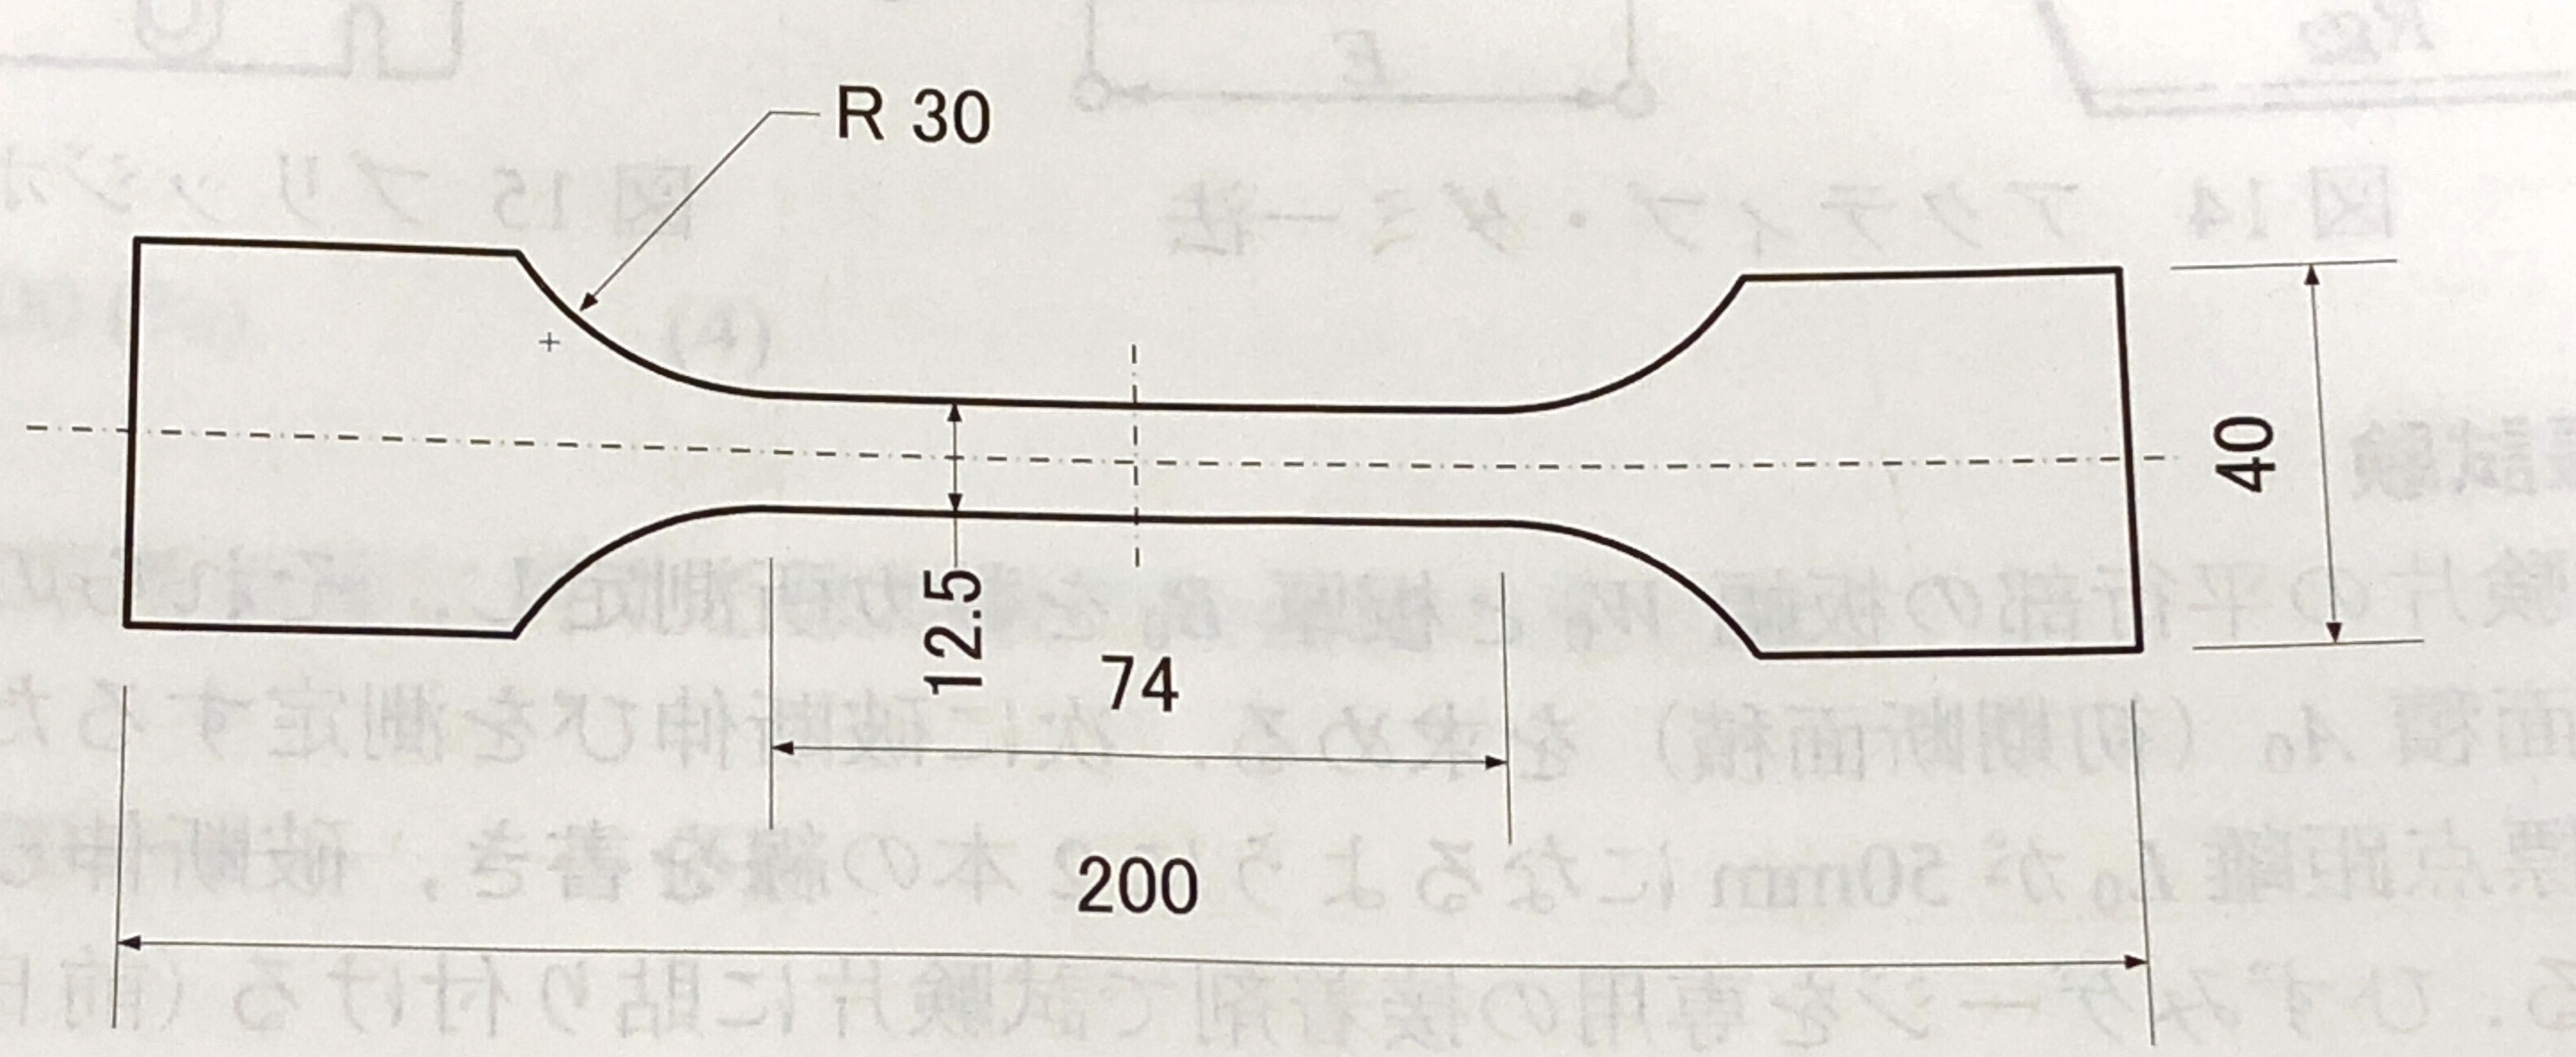
\includegraphics[width = 10cm]{画像/試験片.jpg}
    \caption{試験片の形状寸法}
    \label{試験片}
  \end{center}
\end{figure}

\subsection{縦弾性係数(ヤング率)の測定}
供試材の縦弾性係数を求めるために,試験片標点間の中央付近にひずみゲージを専用の接着剤を用いて貼った.
ひずみゲージは, 共和電業製でベース長9.4mm,ベース幅2.8mm,グリッド長5mm,グリッド幅1.4mmのKFG-5-120-C1を用いた.
ひずみゲージの外観図を図\ref{ひずみげーじ}に示す.

\begin{figure}[H]
  \begin{center}
    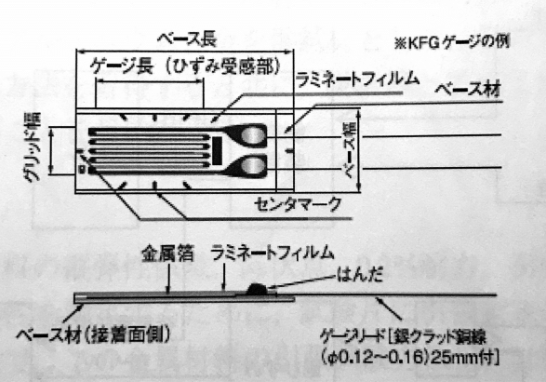
\includegraphics[width = 10cm]{画像/ひずみゲージ.png}
    \caption{ひずみゲージの外観図}
    \label{ひずみげーじ}
  \end{center}
\end{figure}

ひずみゲージは試験片の標点部の「ひずみ」を電気信号として検出するセンサーである.ひずみゲージでブリッジ回路を構成する場合には,
測定目的に応じて1,2,4ゲージ法がある.今回の引張試験では2ゲージ法を用い,1枚をアクティブゲージ,他の1枚を温度補償用のダミーゲージとする(アクティブ・ダミー法).
図\ref{アクティブダミー}にアクティブ・ダミー法の略図を示す.
\par
ひずみの測定は図\ref{試験機}に示すように, アクティブゲージとダミーゲージをブリッジボックスに配線(図\ref{ブリッジボックス})→ブリッジボックスの出力を動ひずみ測定器で増幅
→A/Dコンバータでアナログ信号をデジタル信号に変換→パーソナルコンピュータで集録するという手順で行った.

\begin{figure}[H]
  \begin{center}
    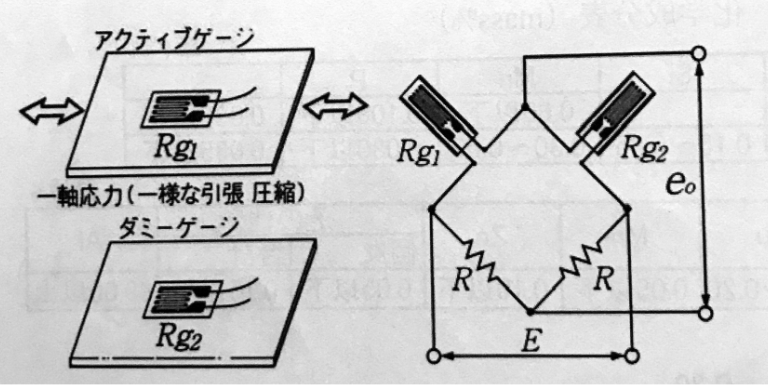
\includegraphics[width = 10cm]{画像/アクティブダミー.png}
    \caption{アクティブ・ダミー}
    \label{アクティブダミー}
  \end{center}
\end{figure}

\begin{figure}[H]
  \begin{center}
    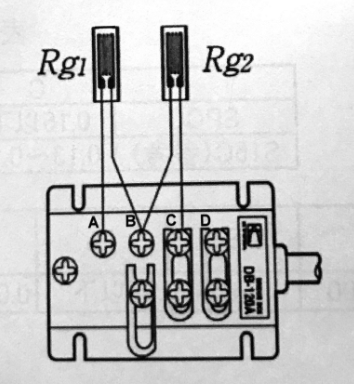
\includegraphics[width = 7cm]{画像/ブリッジボックス.png}
    \caption{ブリッジボックス配線}
    \label{ブリッジボックス}
  \end{center}
\end{figure}

\subsection{引張試験}
\begin{enumerate}
  \item 各試験片の平行部の板幅$W_0$と厚さ$B_0$を数箇所測定し,それらの平均値を用いて原断面積$A_0$(初期断面積)を求めた.
  次に破断伸びを測定するために試験片平行部に標点間距離$L_0$が50mmになるように2本の線を書き,破断伸びを測定する基準とした.
  ひずみゲージはあらかじめ専用の接着剤で試験片に貼付けておいた.
  \item 試験片の上部の掴み部を試験機のチャックに取り付けた.
  \item ひずみゲージの配線を行った.
  \item 試験片の下部の掴み部を試験機のチャックに取り付けた.その際,引張荷重,圧縮荷重が付加されないように試験機のクロスヘッドを微動させながらチャックに取り付けた.
  \item クロスヘッド速度1.0mm/minで引っ張り試験を行った.引張試験で,荷重$P$,クロスヘッドの変位$L$,ひずみゲージから求めたひずみ$\varepsilon$を2台のPCで測定した.
  \item 引張試験終了後,破断部の板厚$W_f$,板幅$B_f$の測定を数カ所行い, それらの平均値を用いて破断ぶの断面積$A_f$を求めた.
  さらに試験片の破断面を付合わせて破断後の標点間距離$L_f$を測定した.
  \item 荷重$P$-変位$L$の関係から,公称応力$\sigma$-公称ひずみ$\varepsilon$線図,真応力$\sigma_t$-真ひずみ$\varepsilon_t$線図を作成した.
  公称応力$\sigma$-公称ひずみ$\varepsilon$線図から上降伏点,下降伏点,引張強さを求めた,さらに破断伸び,破断絞りも求めた
  \item 真応力$\sigma_t$-真ひずみ$\varepsilon_t$線図は\ref{9式}式を用いて公称ひずみ$\varepsilon$から真ひずみ$\varepsilon_t$を計算した.
  真応力$\sigma_t$は最大応力(引張強さ)までは,\ref{7式}式を用いて公称応力$\sigma$と公称ひずみ$\varepsilon$から真応力$\sigma_t$を計算した.
  最大応力(引張強さ)以降は試験片にくびれが発生するため\ref{6式}式が成立しない.したがって, 破断時の荷重$P_f$と破断部の断面積$A_f$から
  破断時の真応力$\sigma_{tf}$を求めて真応力$\sigma_t$-真ひずみ$\varepsilon_t$線図上に破断時の真応力$\sigma_{tf}$をプロットした.
  次に\ref{7式}式から求めた最大応力(引張強さ)までの真応力$\sigma_t$と破断時の真応力$\sigma_{tf}$の間は,図\ref{鋼のひずみ}を参考にフリーハンドで曲線を描き繋いだ.
  \item ひずみゲージから求めたひずみ$\varepsilon$を用いて,公称応力$\sigma$-公称ひずみ$\varepsilon$線図を作成し,縦弾数係数(ヤング率)の計算を行った.
  またA1100の場合,0.2\%耐力もこの公称応力$\sigma$-公称ひずみ$\varepsilon$線図から求めた.
  \item 機械的特性を求めるために用いた計算式を以下に示す.
  \begin{description}
    \item [公称応力$\sigma$]
    \begin{align}
      \sigma = \frac{P}{A_0}
    \end{align}
    \item [公称ひずみ$\varepsilon$]
    \begin{align}
      \varepsilon = \frac{L-L_0}{L_0}
    \end{align}
    \item [破断伸び$\delta$]
    \begin{align}
      \delta = \frac{L_f-L_0}{L_0} \times 100(\%)
    \end{align}
    \item [破断絞り$\varphi$]
    \begin{align}
      \varphi = \frac{A_0-A_f}{A_0} \times 100(\%)
    \end{align}
    \item [真応力$\sigma_t$] \\ 
    引張試験の時, 試験片の負荷荷重が大きくなると, 試験片は伸びて, 板厚$W$と板幅$B$は減少する. 時々刻々の試験片の板厚と板幅から求めた応力を真応力$\sigma_t$
    という. 試験片平行部が均一に変形している状態では,試験片の初期断面積$A_0$,初期標点間距離$L_0$,ある時点での断面積$A$,
    ある点における標点距離$L$の間には以下の関係が成立する.
    \begin{align}
      \label{6式}
      A_0L_0 = AL
    \end{align}
    したがって, 真応力$\sigma_t$は,
    \begin{align}
      \label{7式}
      \sigma_t = \frac{P}{A} = \frac{P}{A_0}\frac{L}{L_0} = \sigma(1+\varepsilon)
    \end{align}
    となる. これより真応力$\sigma_t$は公称応力$\sigma$より大きくなることがわかる.
    \item [真ひずみ$\varepsilon_t$] \mbox{} \\
    ひずみも時々刻々の標点間距離を元にひずみの増加量を定義したのものを真ひずみ$\varepsilon_t$という.ある時点における標点間距離を$L$,
    微小伸びを$dL$, ひずみの増加を$d\varepsilon$とすると次のようになる.
    \begin{align}
      d\varepsilon = \frac{dl}{l}
    \end{align}
    これを$L_0$から$L$まで積分すると,
    \begin{align}
      \label{9式}
      \varepsilon_t = \int_{L_0}^L \frac{dl}{l} = \log \left(1+\frac{L-L_0}{L_0}\right) = \log(1+\varepsilon)
    \end{align}
  \end{description}
\end{enumerate}
\section{実験結果と考察}
\subsection{金属材料の組織観察}
極軟鋼,S15C,S45C,SK85(SK5),SK105(SK3)のNo.22から32までの各組織の画像を以下の図\ref{極なまし}〜\ref{SK105焼入れ焼戻し}に示す.

\begin{figure}[H]
  \begin{tabular}{cc}
    \begin{minipage}{0.5\hsize}
      \begin{center}
        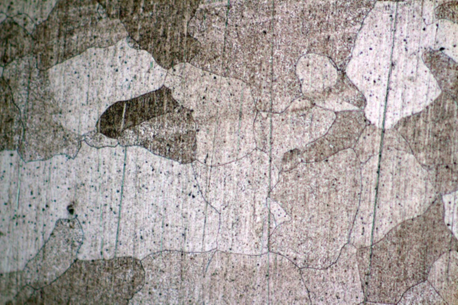
\includegraphics[width = 5cm]{画像/極なまし.png}
        \caption{No.22 極軟鋼 焼なまし (倍率:200)}
        \label{極なまし}
      \end{center}
    \end{minipage}

    \begin{minipage}{0.5\hsize}
      \begin{center}
        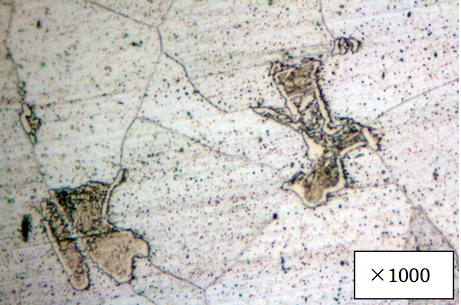
\includegraphics[width = 5cm]{画像/S15Cなまし.png}
        \caption{No.23 S15C 焼なまし (倍率:1000)}
        \label{S15Cなまし}
      \end{center}
    \end{minipage}
  \end{tabular}
\end{figure}

\begin{figure}[H]
  \begin{tabular}{cc}
    \begin{minipage}{0.5\hsize}
      \begin{center}
        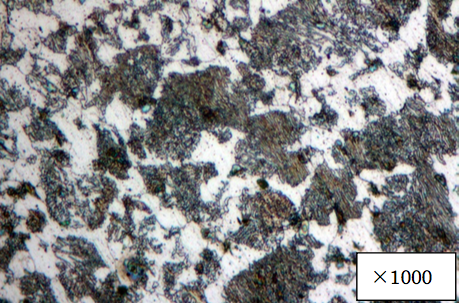
\includegraphics[width = 5cm]{画像/S45Cなまし.png}
        \caption{No.24 S45C 焼なまし (倍率:1000)}
        \label{S45C焼なまし}
      \end{center}
    \end{minipage}

    \begin{minipage}{0.5\hsize}
      \begin{center}
        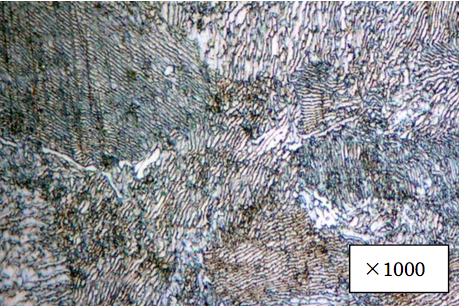
\includegraphics[width = 5cm]{画像/SK85なまし.png}
        \caption{No.27 SK85 焼なまし (倍率:1000)}
        \label{SK85なまし}
      \end{center}
    \end{minipage}
  \end{tabular}
\end{figure}

\begin{figure}[H]
  \begin{tabular}{cc}
    \begin{minipage}{0.5\hsize}
      \begin{center}
        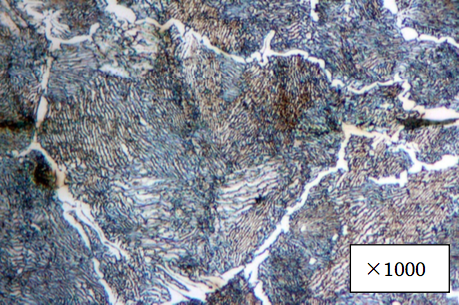
\includegraphics[width = 5cm]{画像/SK105なまし.png}
        \caption{No.30 SK105 焼なまし (倍率:1000)}
        \label{SK105焼なまし}
      \end{center}
    \end{minipage}

    \begin{minipage}{0.5\hsize}
      \begin{center}
        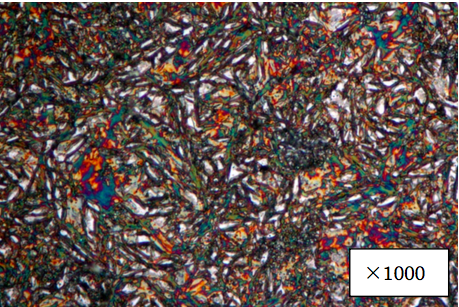
\includegraphics[width = 5cm]{画像/SK105焼入れ.png}
        \caption{No.31 SK105 焼入れ (倍率:1000)}
        \label{SK105焼入れ}
      \end{center}
    \end{minipage}
  \end{tabular}
\end{figure}

\begin{figure}[H]
      \begin{center}
        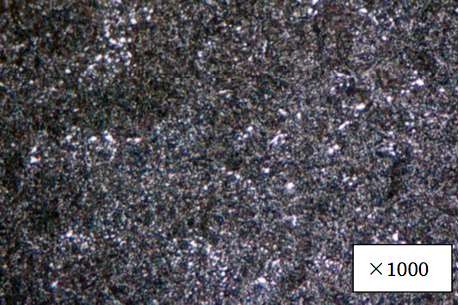
\includegraphics[width = 5cm]{画像/SK105焼入れ焼戻し.png}
        \caption{No.32 SK105 焼入れ焼戻し (倍率:1000)}
        \label{SK105焼入れ焼戻し}
      \end{center}
\end{figure}



\subsubsection{熱処理による相変態過程と観察した組織についての説明}
\begin{description}
  \item[No.22 極軟鋼 焼なまし]
  まず$A_3$線を上回る温度まで上げ全てオーステナイトになった後, 炉冷していくと$A_3$線上からフェライトの析出が始まる(初析フェライト). さらに温度が低下するとオーステナイトは減少し,
  フェライトが次第に増加し, ほとんどがフェライトになる. 図\ref{極なまし}を見ると, 全体的に白色の組織が占めており, これがフェライトである.
  \item[No.23 S15C 焼なまし]
  まず$A_3$線を上回る温度まで上げ全てオーステナイトになった後, 炉冷していくと$A_3$線上からフェライトの析出が始まる. さらに温度が低下するとオーステナイトは減少し,
  フェライトが次第に増加していく, さらに低下させ$A_1$線を下回るとセメンタイトが析出し始め, セメンタイトと未変態のオーステナイトによる共析変態が起こり,
  最終的にフェライトとパーライトの混合組織になる.
  図\ref{S15Cなまし}を見ると, 白色のフェライトの中に黒色のパーライト組織があることがわかる.
  \item[No.24 S45C 焼なまし]
  まず$A_3$線を上回る温度まで上げ全てオーステナイトになった後, 炉冷していくと$A_3$線上からフェライトの析出が始まる. さらに温度が低下するとオーステナイトは減少し,
  フェライトが次第に増加していく, さらに低下させ$A_1$線を下回るとセメンタイトが析出し始め, セメンタイトと未変態のオーステナイトによる共析変態が起こり,
  最終的にフェライトとパーライトの混合組織になる. 図\ref{S45C焼なまし}を見ると, 白色フェライトと黒色パーライトの混合組織が見て取れる.
  S15Cの場合と比較すると, パーライトの割合が増え, 所々層状の組織が見られる.
  \item[No.27 SK85 焼なまし]
  まず$A_3$線を上回る温度まで上げ全てオーステナイトになった後, 炉冷していき, $A_1$線を下回るとオーステナイトはフェライトとセメンタイトに分解する共析変態が起こり,
  全てパーライトとなる. 図\ref{SK85なまし}を見ると, 全体的に層状のパーライト組織が占めているのが見て取れる.
  \item[No.30 SK105 焼なまし]
  まず$A_{cm}$線を上回る温度まで上げ全てオーステナイトになった後, 炉冷していくと$A_{cm}$線上から
  セメンタイトがオーステナイトの粒界に網目状に析出を始める(初析セメンタイト). さらに温度が低下すると, セメンタイトは増加し, $A_1$戦場から未変態のオーステナイトが共析変態を起こしてパーライトとなる.
  最終的には網目状のセメンタイトとパーライトの組織となる. 図\ref{SK105焼なまし}を見ると, 層状のパーライト組織が全体を占めており, 所々に黒色のセメンタイトの線状組織が確認できる.
  \item[No.31 SK105 焼入れ]
  まず$A_{cm}$線を上回る温度まで上げ全てオーステナイトになった後, $A_1$線を下回るまで急冷させると, オーステナイトは無拡散変態を起こし, マルテンサイト組織となる.
  この時, オーステナイトが残留するが, 時間と共にマルテンサイト化する. 図\ref{SK105焼入れ}を見ると, 全体に針状の組織が分布しており, マルテンサイトが確認できる.
  \item[No.32 SK105 焼入れ焼戻し]
  まず$A_{cm}$線を上回る温度まで上げ全てオーステナイトになった後, $A_1$線を下回るまで急冷させると, オーステナイトは無拡散変態を起こし, マルテンサイト組織となる.
  その後, $A_1$線直下まで再加熱し, 冷却すると, 粒状のソルバイト組織となる. 図\ref{SK105焼入れ焼戻し}を見ると, 全体に黒色粒状のマルテンサイト組織が広がっているのが確認できる.
\end{description}
\subsubsection{炭素量の増加と標準組織の変化について}
炭素量と標準組織の関係について説明する.実験で観察したNo.22,23,24,27,30の試料を比較すると,極軟鋼では大部分がフェライトで構成されているが, No.23,24,27,30と炭素量が増加するにつれパーライトの割合が多くなり,
No.27, つまりSK85ではほぼ全体の組織がパーライトになる.SK105(No.30)ではさらに炭素量が増加し, セメンタイトが多く析出している.

\subsubsection{焼入れ焼もどしの目的とマルテンサイト変態, 残留オーステナイトについて}
焼入れ,焼もどしの目的とマルテンサイト変態,残留オーステナイトについて説明する.
\par
焼入れとは,鉄鋼を均一オーステナイト状態になるまで加熱し,
この温度で一定時間保持した後,水などを用いて急冷する熱処理である.これにより, オーステナイトの大部分は無拡散変態により, フェライトやパーライトへは変態せず, マルテンサイト変態が起こる.
マルテンサイト組織によって硬度が上がり, またこれによって焼割れや焼ひずみが生じなくなる.これが焼入れの目的である.
しかしながら, 焼入れした鉄鋼は固いものの, 脆いために実製品として使用することは難しい.
\par
焼戻しとは, 焼入れした鉄鋼をオーステナイトを生じない温度まで再加熱し, 一定時間保持した後, 徐々に温度を低下させていき, ソルバイト組織を生じさせることである.
焼戻しの目的は, 硬いが脆い焼入れ材に粘り強さを与えることや, マルテンサイト化した残留オーステナイトを安定させる目的がある.
靱性を重視する場合は比較的高温で焼戻しする高温焼戻しが、硬さを重視する場合は比較的低温で焼戻しする低温焼戻しが適用される.
焼戻し温度によって, 適切でない冷却方法を選択してしまうと, 反対に脆くなってしまう焼戻し脆性が生じることがある.
\par
マルテンサイト変態とは, 鉄鋼を均一オーステナイト状態になるまで加熱し, 一定時間温度を保持した鉄鋼を臨界冷却速度を上回る速さで急冷することにより,オーステナイトの大部分が無拡散変態により,
マルテンサイトに変態することである.マルテンサイトは非常に硬inline針状の組織で,マルテンサイトが多いほど鉄鋼の硬度は上がる.
\par
残留オーステナイトとは, 焼入れによって鉄鋼をを急冷させ, マルテンサイト変態が起きる時に, マルテンサイト変態をせずに残ってしまうオーステナイトのことである.
実際には数\%から30\%のオーステナイトはマルテンサイトに変態せずオーステナイトのまま室温に達する.残留オーステナイトは室温では不安定な組織であるため,長時間経過するとマルテンサイト化する.

\subsection{金属材料の引張試験}
\subsubsection{SPCCとA1100の引張試験から得られた荷重$P$と伸び$L$のデータから, 公称応力$\sigma$-公称ひずみ$\varepsilon$線図, 真応力$\sigma_t$-真ひずみ$\varepsilon_t$線図を作成する.}
引張試験前後の試料の標点間距離, 板幅, 板厚の計測結果を以下の表\ref{試料1},\ref{試料2}に示す. また,それらの計測結果と引張試験の実験データから得られたSPCCとA1100の
公称応力$\sigma$-公称ひずみ$\varepsilon$線図を図\ref{SPCC公称線図},\ref{A1100公称線図}に, 真応力$\sigma_t$-真ひずみ$\varepsilon_t$線図を図\ref{SPCC真線図}, \ref{A1100真線図},に示した.

\begin{table}[H]
\begin{center}
\caption{各試料の測定値(実験前)}
\label{試料1}
\begin{tabular}{|l|l|l|l|} \hline
試料    & 標点間距離 $L_0$[mm] & 板幅 $W_0$[mm] & 板厚 $B_0$[mm]\\ \hline
SPCC  & 47.76        & 12.13 & 1.73 \\
A1100 & 48.1         & 12.38 & 1.98 \\ \hline
\end{tabular}
\end{center}
\end{table}

\begin{table}[H]
\begin{center}
\caption{各試料の測定値(破断時)}
\label{試料2}
\begin{tabular}{|l|l|l|l|} \hline
  試料    & 標点間距離 $L_f$[mm] & 板幅 $W_f$[mm] & 板厚 $B_f$[mm] \\ \hline
  SPCC  & 71.0         & 6.88      & 0.767    \\
  A1100 & 54.6         & 9.55      & 0.616  \\ \hline
\end{tabular}
\end{center}
\end{table}

\begin{figure}[H]
      \begin{center}
        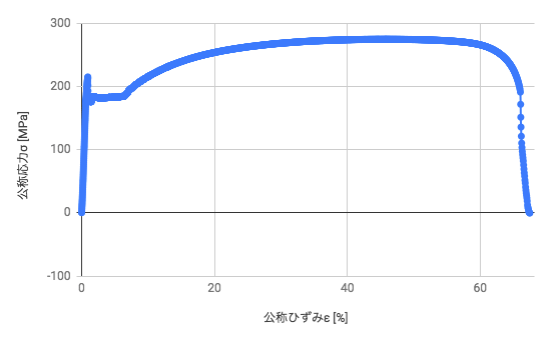
\includegraphics[width = 10cm]{画像/公称線図.png}
        \caption{試験機の荷重と変位から求めたSPCCの公称応力$\sigma$-公称ひずみ$\varepsilon$線図}
        \label{SPCC公称線図}
      \end{center}
\end{figure}

\begin{figure}[H]
      \begin{center}
        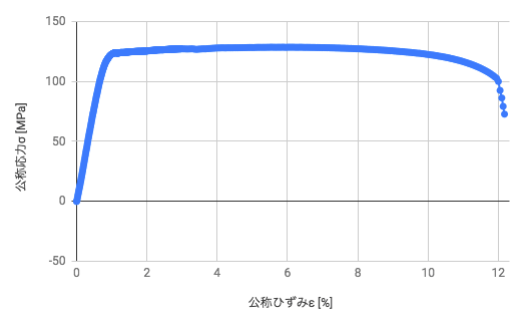
\includegraphics[width = 10cm]{画像/A1100公称線図.png}
        \caption{試験機の荷重と変位から求めたA1100の公称応力$\sigma$-公称ひずみ$\varepsilon$線図}
        \label{A1100公称線図}
      \end{center}
\end{figure}

\begin{figure}[H]
      \begin{center}
        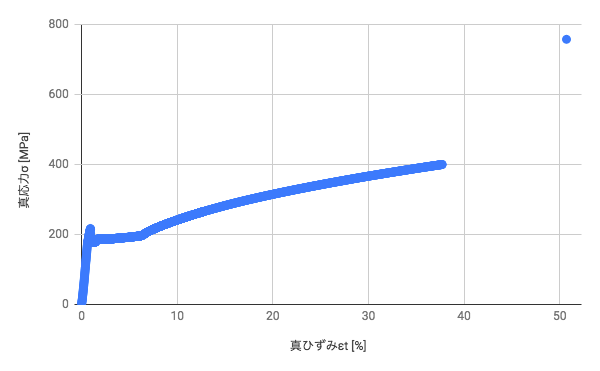
\includegraphics[width = 10cm]{画像/真応力.png}
        \caption{試験機の荷重と変位から求めたSPCCの真応力$\sigma$-真ひずみ$\varepsilon$線図}
        \label{SPCC真線図}
      \end{center}
\end{figure}

\begin{figure}[H]
      \begin{center}
        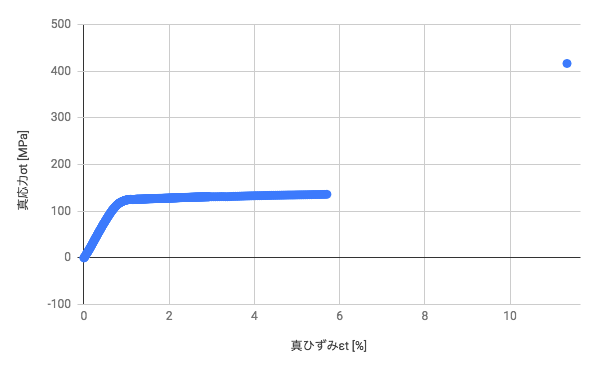
\includegraphics[width = 10cm]{画像/真応力2.png}
        \caption{試験機の荷重と変位から求めたA1100の真応力$\sigma_t$-真ひずみ$\varepsilon_t$線図}
        \label{A1100真線図}
      \end{center}
\end{figure}

\subsubsection{機械的特性として, 縦弾性係数, 降伏点(SPCC: 上降伏点と下降伏点) または0.2\%耐力(A1100), 引張強さ, 破断強さ, 破断伸び, 破断絞りを求める.}
SPCCとA1100の機械的特性として縦弾性係数,降伏点(SPCC:上降伏点と下降伏点), 0.2\%耐力(A1100),引張強さ,破断強さ,破断伸びおよび破断絞りを求める.
縦弾性係数は以下に示すひずみゲージから求めた公称応力$\sigma$-公称ひずみ$\varepsilon$線図から得られた.
また.A1100の0.2\%耐力は, 傾きが縦弾性係数に等しくx軸との交点が0.002である直線と公称応力$\sigma$-公称ひずみ$\varepsilon$線図の交点から求めた.
以上の結果を表\ref{実験結果1}, \ref{実験結果2}にまとめた.

\begin{figure}[H]
      \begin{center}
        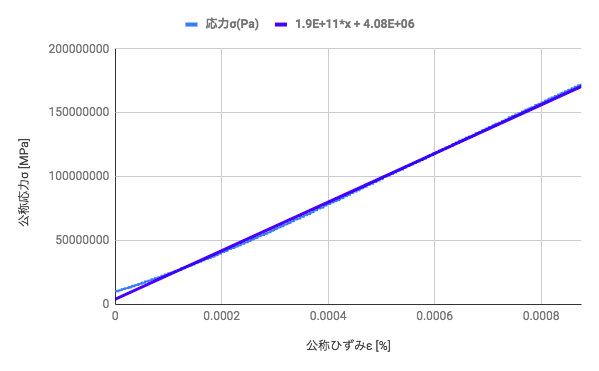
\includegraphics[width = 10cm]{画像/SPCCひずみゲージ.png}
        \caption{ひずみゲージから求めたSPCCの公称応力$\sigma$-公称ひずみ$\varepsilon$線図}
        \label{SPCCひずみゲージ}
      \end{center}
\end{figure}

\begin{figure}[H]
      \begin{center}
        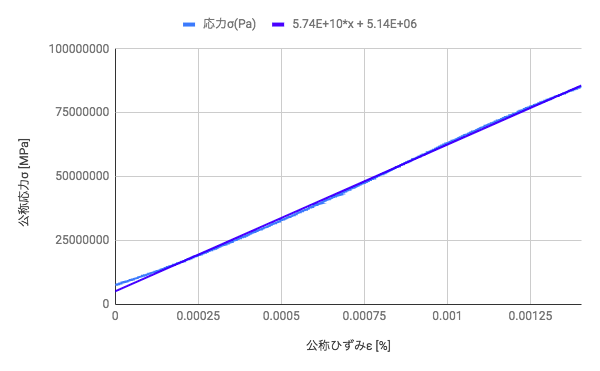
\includegraphics[width = 10cm]{画像/A1100ひずみゲージ.png}
        \caption{ひずみゲージから求めたA1100の公称応力$\sigma$-公称ひずみ$\varepsilon$線図}
        \label{A1100ひずみゲージ}
      \end{center}
\end{figure}

\begin{figure}[H]
      \begin{center}
        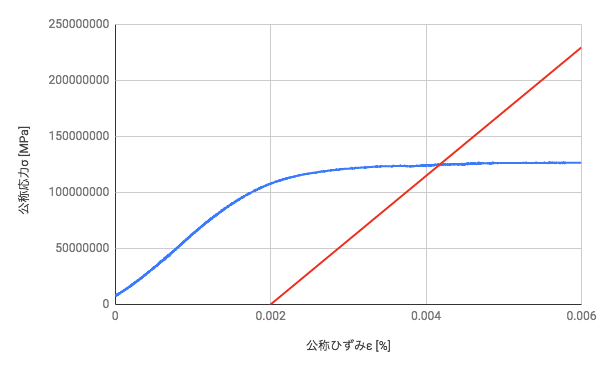
\includegraphics[width = 10cm]{画像/耐力.png}
        \caption{ひずみゲージから求めたA1100の公称応力$\sigma$-公称ひずみ$\varepsilon$線図(0.2\%耐力計算用)}
        \label{0.2耐力}
      \end{center}
\end{figure}


\begin{table}[H]
\begin{center}
\caption{各グラフから得られた実験結果(1)}
\label{実験結果1}
  \begin{tabular}{|l|l|l|l|l|}
  \hline
  試料    & 縦弾数係数 [GPa] & 引張強さ [MPa] & 破断強さ [MPa] & 破断伸び [\%] \\ \hline
  SPCC  & 190             & 274.4          & 190.8          & 48.5          \\
  A1100 & 57.4            & 128.5          & 99.9           & 13.5          \\ \hline
  \end{tabular}
\end{center}
\end{table}

\begin{table}[H]
\begin{center}
  \caption{各グラフから得られた実験結果(2)}
  \label{実験結果2}
  \begin{tabular}{|l|l|l|l|l|}
  \hline
  試料    & 破断絞り [\%]& 上降伏点 [MPa]& 下降伏点 [MPa]& 0.2\%耐力 [MPa]\\ \hline
  SPCC  & 76.2 & 214.9 & 181.2 & -       \\
  A1100 & 76.0 & -     & -     & 127.6   \\ \hline
  \end{tabular}
\end{center}
\end{table}

\subsubsection{SPCCとA1100の機械的特性の違いについて}
実験から得られたそれぞれの結果から, SPCCとA1100の機械的特性について考察する.
\begin{description}
  \item[縦弾数係数]
  縦弾数係数を比較すると, SPCCは190[GPa], A1100は57.4[GPa], つまりSPCCはA1100の3.31倍となっていることから, SPCCはA1100に比べてかなり伸びにくい材料であり, 逆にA1100はSPCCに比べて伸びやすい性質であることがわかった.
  \item[引張強さ]
  引張強さを比較すると, SPCCは274.4[MPa], A1100は128.5[MPa], つまりSPCCはA1100の2.14倍となっていることから, SPCCはA1100に比べると引張力に対して約2.14倍の最大強度があることがわかった.
  \item[破断強さ]
  破断強さを比較すると, SPCCは190.8[MPa], A1100は99.9[MPa], つまりSPCCはA1100の1.91倍となっていることから, SPCCはA1100に比べると引張力に対して約1.91倍の破断時の強度があることがわかった.
  \item[破断伸び]
  破断伸びを比較すると, SPCCは48.5[\%], A1100は13.5[\%], つまりSPCCはA1100の3.59倍となっていることから, SPCCはA1100に比べると破断までに3.59倍伸び, SPCCの方が伸びやすいことがわかった.
  \item[破断絞り]
  破断絞りを比較すると, SPCCは76.2[\%], A1100は76.0[\%], つまりSPCCはA1100の1.00倍となっていることから, 破断時の絞りはSPCCもA1100も同等であることがわかった.
  \item[降伏点]
  降伏点を比較すると, SPCCの上降伏点は181.2[MPa], A1100の0.2\%耐力は127.6[MPa], つまりSPCCはA1100の1.42倍となっていることから, SPCCはA1100に比べると降伏までに約1.42倍の強度があることがわかった.
\end{description}

\section{参考文献}
\begin{thebibliography}{9}
  \bibitem{s1} 知能機械工学基礎実験, 電気通信大学  知能機械工学科
\end{thebibliography}
\end{document}
